\section*{Our Result}

原始圖片:
\begin{figure}[!ht]
    \centering
    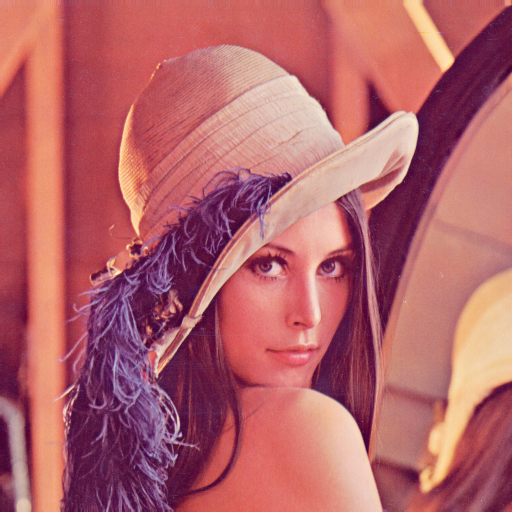
\includegraphics[width=0.22\linewidth]{../images/samples/lena.png}
\end{figure}

\subsection*{Basic Operations}

下圖比較我們實作後由不同模式進行 morphological operations 的結果。
\begin{figure}[!ht]
   \centering
\begin{subfigure}[t]{0.22\textwidth}
    \includegraphics[width=0.9\linewidth]{../images/outputs/compare\_mode1/dilation\_sum.png}
    \caption{dilation with sum}
    \centering
  \end{subfigure}
\begin{subfigure}[t]{0.22\textwidth}
    \includegraphics[width=0.9\linewidth]{../images/outputs/compare\_mode1/erosion\_sum.png}
    \caption{erosion with sum}
    \centering
  \end{subfigure}
\begin{subfigure}[t]{0.22\textwidth}
    \includegraphics[width=0.9\linewidth]{../images/outputs/compare\_mode1/opening\_sum.png}
    \caption{opening with sum}
    \centering
  \end{subfigure}
\begin{subfigure}[t]{0.22\textwidth}
    \includegraphics[width=0.9\linewidth]{../images/outputs/compare\_mode1/closing\_sum.png}
    \caption{closing with sum}
    \centering
  \end{subfigure}
\begin{subfigure}[t]{0.22\textwidth}
    \includegraphics[width=0.9\linewidth]{../images/outputs/compare\_mode1/dilation\_prod.png}
    \caption{dilation with product}
    \centering
  \end{subfigure}
\begin{subfigure}[t]{0.22\textwidth}
    \includegraphics[width=0.9\linewidth]{../images/outputs/compare\_mode1/erosion\_prod.png}
    \caption{erosion with product}
    \centering
  \end{subfigure}
\begin{subfigure}[t]{0.22\textwidth}
    \includegraphics[width=0.9\linewidth]{../images/outputs/compare\_mode1/opening\_prod.png}
    \caption{opening with product}
    \centering
  \end{subfigure}
\begin{subfigure}[t]{0.22\textwidth}
    \includegraphics[width=0.9\linewidth]{../images/outputs/compare\_mode1/closing\_prod.png}
    \caption{closing with product}
    \centering
  \end{subfigure}
\begin{subfigure}[t]{0.22\textwidth}
    \includegraphics[width=0.9\linewidth]{../images/outputs/compare\_mode1/dilation\_median.png}
    \caption{dilation with median}
    \centering
  \end{subfigure}
\begin{subfigure}[t]{0.22\textwidth}
    \includegraphics[width=0.9\linewidth]{../images/outputs/compare\_mode1/erosion\_median.png}
    \caption{erosion with median}
    \centering
  \end{subfigure}
\begin{subfigure}[t]{0.22\textwidth}
    \includegraphics[width=0.9\linewidth]{../images/outputs/compare\_mode1/opening\_median.png}
    \caption{opening with median}
    \centering
  \end{subfigure}
\begin{subfigure}[t]{0.22\textwidth}
    \includegraphics[width=0.9\linewidth]{../images/outputs/compare\_mode1/closing\_median.png}
    \caption{closing with median}
    \centering
  \end{subfigure}
 \caption{Comparison of different modes}
 \end{figure}

以視覺上而言並無明顯差異,和論文一致。

接著比較使用不同大小的 structuring element 進行 morphological operations 的結果。
\begin{figure}[!ht]
    \centering
    \begin{subfigure}{0.9\textwidth}
   \centering
\begin{subfigure}[t]{0.22\textwidth}
    \includegraphics[width=0.9\linewidth]{../images/outputs/erosion\_exp/lena\_erosion1.png}
    
    \centering
  \end{subfigure}
\begin{subfigure}[t]{0.22\textwidth}
    \includegraphics[width=0.9\linewidth]{../images/outputs/erosion\_exp/lena\_erosion3.png}
    
    \centering
  \end{subfigure}
\begin{subfigure}[t]{0.22\textwidth}
    \includegraphics[width=0.9\linewidth]{../images/outputs/erosion\_exp/lena\_erosion5.png}
    
    \centering
  \end{subfigure}
 \caption{erosion with different SE}
 \end{subfigure}

    \begin{subfigure}{0.9\textwidth}
   \centering
\begin{subfigure}[t]{0.22\textwidth}
    \includegraphics[width=0.9\linewidth]{../images/outputs/dilation\_exp/lena\_dilation1.png}
    
    \centering
  \end{subfigure}
\begin{subfigure}[t]{0.22\textwidth}
    \includegraphics[width=0.9\linewidth]{../images/outputs/dilation\_exp/lena\_dilation3.png}
    
    \centering
  \end{subfigure}
\begin{subfigure}[t]{0.22\textwidth}
    \includegraphics[width=0.9\linewidth]{../images/outputs/dilation\_exp/lena\_dilation5.png}
    
    \centering
  \end{subfigure}
 \caption{dilation with different SE}
 \end{subfigure}

    \caption{morphological operations with different structuring element size}
\end{figure}
可看出,隨著 structuring element size 的增加,圖片的變化也越來越明顯。

\clearpage
我們也嘗試了另一種 ordering 的方法作為參照:先將圖片轉為 HSV,接著以 $(V, S, H)$ 的順位進行比較。此外也附上轉為灰階後 morphological operations 的結果。

\begin{figure}[!ht]
   \centering
\begin{subfigure}[t]{0.22\textwidth}
    \includegraphics[width=0.9\linewidth]{../images/outputs/compare\_order/dilation\_proposed.png}
    \caption{dilation with proposed}
    \centering
  \end{subfigure}
\begin{subfigure}[t]{0.22\textwidth}
    \includegraphics[width=0.9\linewidth]{../images/outputs/compare\_order/dilation\_proposed\_fuzzy.png}
    \caption{dilation with proposed (fuzzy)}
    \centering
  \end{subfigure}
\begin{subfigure}[t]{0.22\textwidth}
    \includegraphics[width=0.9\linewidth]{../images/outputs/compare\_order/erosion\_proposed.png}
    \caption{erosion with proposed}
    \centering
  \end{subfigure}
\begin{subfigure}[t]{0.22\textwidth}
    \includegraphics[width=0.9\linewidth]{../images/outputs/compare\_order/erosion\_proposed\_fuzzy.png}
    \caption{erosion with proposed (fuzzy)}
    \centering
  \end{subfigure}
\begin{subfigure}[t]{0.22\textwidth}
    \includegraphics[width=0.9\linewidth]{../images/outputs/compare\_order/dilation\_HSV.png}
    \caption{dilation with HSV}
    \centering
  \end{subfigure}
\begin{subfigure}[t]{0.22\textwidth}
    \includegraphics[width=0.9\linewidth]{../images/outputs/compare\_order/dilation\_HSV\_fuzzy.png}
    \caption{dilation with HSV (fuzzy)}
    \centering
  \end{subfigure}
\begin{subfigure}[t]{0.22\textwidth}
    \includegraphics[width=0.9\linewidth]{../images/outputs/compare\_order/erosion\_HSV.png}
    \caption{erosion with HSV}
    \centering
  \end{subfigure}
\begin{subfigure}[t]{0.22\textwidth}
    \includegraphics[width=0.9\linewidth]{../images/outputs/compare\_order/erosion\_HSV\_fuzzy.png}
    \caption{erosion with HSV (fuzzy)}
    \centering
  \end{subfigure}
\begin{subfigure}[t]{0.22\textwidth}
    \includegraphics[width=0.9\linewidth]{../images/outputs/compare\_order/dilation\_gray scale.png}
    \caption{dilation with gray scale}
    \centering
  \end{subfigure}
\begin{subfigure}[t]{0.22\textwidth}
    \includegraphics[width=0.9\linewidth]{../images/outputs/compare\_order/dilation\_gray scale\_fuzzy.png}
    \caption{dilation with gray scale (fuzzy)}
    \centering
  \end{subfigure}
\begin{subfigure}[t]{0.22\textwidth}
    \includegraphics[width=0.9\linewidth]{../images/outputs/compare\_order/erosion\_gray scale.png}
    \caption{erosion with gray scale}
    \centering
  \end{subfigure}
\begin{subfigure}[t]{0.22\textwidth}
    \includegraphics[width=0.9\linewidth]{../images/outputs/compare\_order/erosion\_gray scale\_fuzzy.png}
    \caption{erosion with gray scale (fuzzy)}
    \centering
  \end{subfigure}
 \caption{Comparison of RGB and HSV orderings}
 \end{figure}


大致效果相似,不過放大觀察可以看出本論文使用的方法在不同顏色交界上最為平滑且保留細節。

\clearpage
\subsection*{Denoising}
首先,我們在圖片中分別加入 $10\%$ 的 salt 及 pepper noise,並分別使用 opening 及 closing 進行 denoising。
\begin{figure}[!ht]
   \centering
\begin{subfigure}[t]{0.25\textwidth}
    \includegraphics[width=0.9\linewidth]{../images/outputs/noise\_exp/lena\_salt.png}
    \caption{salt noise}
    \centering
  \end{subfigure}
\begin{subfigure}[t]{0.25\textwidth}
    \includegraphics[width=0.9\linewidth]{../images/outputs/noise\_exp/lena\_salt\_opening.png}
    \caption{salt noise opening}
    \centering
  \end{subfigure}
\begin{subfigure}[t]{0.25\textwidth}
    \includegraphics[width=0.9\linewidth]{../images/outputs/noise\_exp/lena\_salt\_closing.png}
    \caption{salt noise closing}
    \centering
  \end{subfigure}
\begin{subfigure}[t]{0.25\textwidth}
    \includegraphics[width=0.9\linewidth]{../images/outputs/noise\_exp/lena\_pepper.png}
    \caption{pepper noise}
    \centering
  \end{subfigure}
\begin{subfigure}[t]{0.25\textwidth}
    \includegraphics[width=0.9\linewidth]{../images/outputs/noise\_exp/lena\_pepper\_opening.png}
    \caption{pepper noise opening}
    \centering
  \end{subfigure}
\begin{subfigure}[t]{0.25\textwidth}
    \includegraphics[width=0.9\linewidth]{../images/outputs/noise\_exp/lena\_pepper\_closing.png}
    \caption{pepper noise closing}
    \centering
  \end{subfigure}
 \caption{pepper/salt noise}
 \end{figure}

\clearpage
接著我們在許多圖片加入 $10\%$ impulse noise,並比較 open-closing,close-opening 以及 Wang 等人所提出的 hypergraph 方法 [2]。Wang 的部分為我們參考其原始論文並實作而來。
\begin{figure}[!ht]
    \centering
    \begin{subfigure}{0.9\textwidth}
   \centering
\begin{subfigure}[t]{0.15\textwidth}
    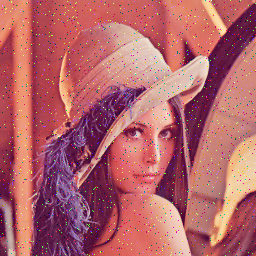
\includegraphics[width=0.9\linewidth]{../images/outputs/denoise/before/before0.png}
    
    \centering
  \end{subfigure}
\begin{subfigure}[t]{0.15\textwidth}
    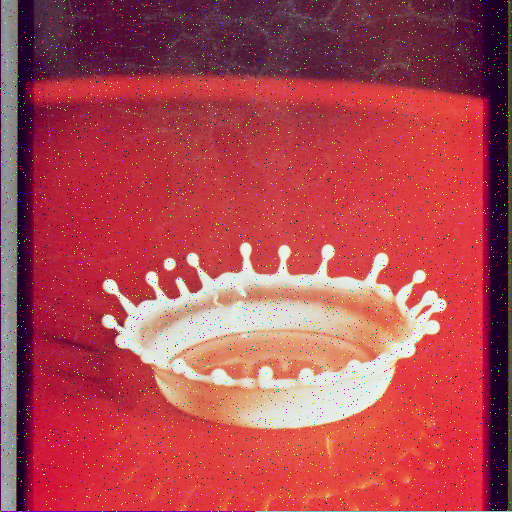
\includegraphics[width=0.9\linewidth]{../images/outputs/denoise/before/before1.png}
    
    \centering
  \end{subfigure}
\begin{subfigure}[t]{0.15\textwidth}
    
\includegraphics[width=0.9\linewidth]{../images/outputs/denoise/before/before2.png}
    
    \centering
  \end{subfigure}
\begin{subfigure}[t]{0.15\textwidth}
    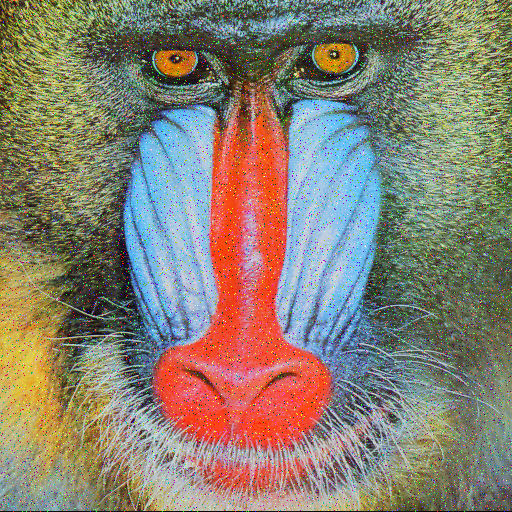
\includegraphics[width=0.9\linewidth]{../images/outputs/denoise/before/before3.png}
    
    \centering
  \end{subfigure}
\begin{subfigure}[t]{0.15\textwidth}
    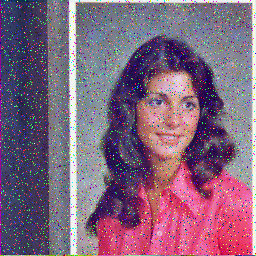
\includegraphics[width=0.9\linewidth]{../images/outputs/denoise/before/before4.png}
    
    \centering
  \end{subfigure}
\begin{subfigure}[t]{0.15\textwidth}
    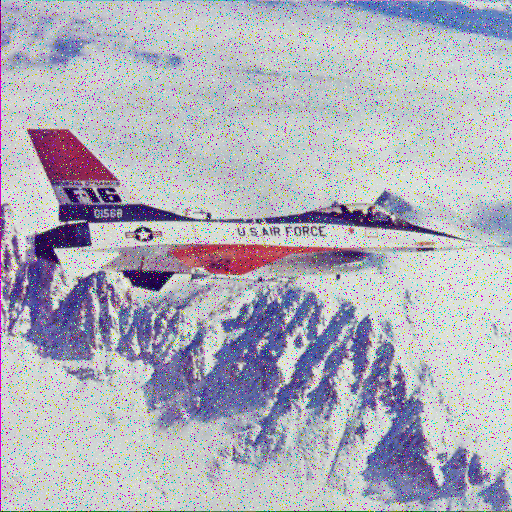
\includegraphics[width=0.9\linewidth]{../images/outputs/denoise/before/before5.png}
    
    \centering
  \end{subfigure}
 \caption{Noisy images}
 \end{subfigure}

    \begin{subfigure}{0.9\textwidth}
   \centering
\begin{subfigure}[t]{0.15\textwidth}
    
\includegraphics[width=0.9\linewidth]{../images/outputs/denoise/co/co0.png}
    
    \centering
  \end{subfigure}
\begin{subfigure}[t]{0.15\textwidth}
    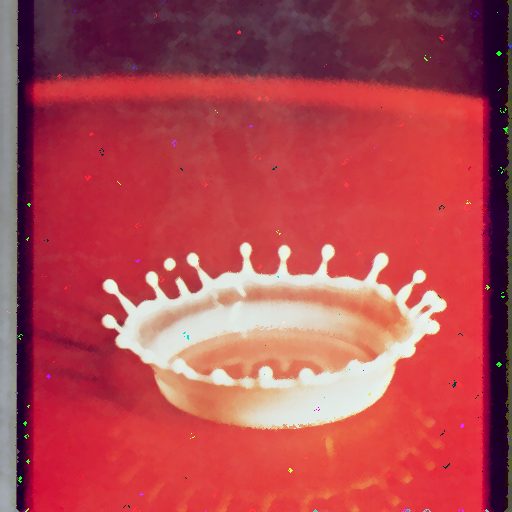
\includegraphics[width=0.9\linewidth]{../images/outputs/denoise/co/co1.png}
    
    \centering
  \end{subfigure}
\begin{subfigure}[t]{0.15\textwidth}
    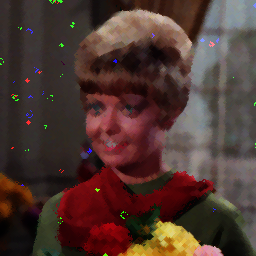
\includegraphics[width=0.9\linewidth]{../images/outputs/denoise/co/co2.png}
    
    \centering
  \end{subfigure}
\begin{subfigure}[t]{0.15\textwidth}
    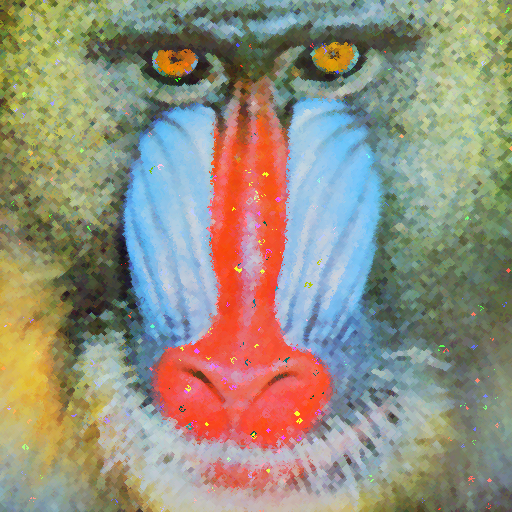
\includegraphics[width=0.9\linewidth]{../images/outputs/denoise/co/co3.png}
    
    \centering
  \end{subfigure}
\begin{subfigure}[t]{0.15\textwidth}
    
\includegraphics[width=0.9\linewidth]{../images/outputs/denoise/co/co4.png}
    
    \centering
  \end{subfigure}
\begin{subfigure}[t]{0.15\textwidth}
    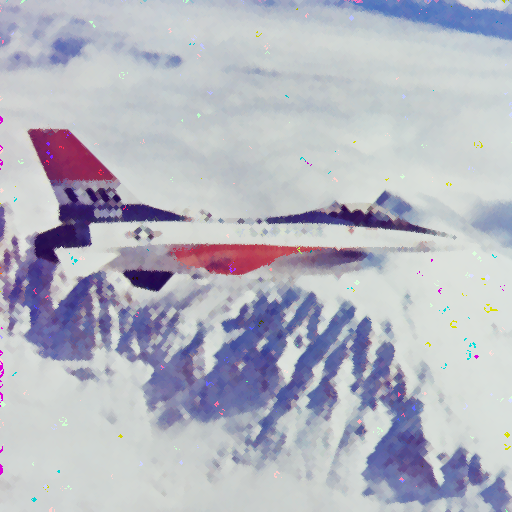
\includegraphics[width=0.9\linewidth]{../images/outputs/denoise/co/co5.png}
    
    \centering
  \end{subfigure}
 \caption{close-opening with proposed method}
 \end{subfigure}

    \begin{subfigure}{0.9\textwidth}
   \centering
\begin{subfigure}[t]{0.15\textwidth}
    
\includegraphics[width=0.9\linewidth]{../images/outputs/denoise/oc/oc0.png}
    
    \centering
  \end{subfigure}
\begin{subfigure}[t]{0.15\textwidth}
    \includegraphics[width=0.9\linewidth]{../images/outputs/denoise/oc/oc1.png}
    
    \centering
  \end{subfigure}
\begin{subfigure}[t]{0.15\textwidth}
    \includegraphics[width=0.9\linewidth]{../images/outputs/denoise/oc/oc2.png}
    
    \centering
  \end{subfigure}
\begin{subfigure}[t]{0.15\textwidth}
    \includegraphics[width=0.9\linewidth]{../images/outputs/denoise/oc/oc3.png}
    
    \centering
  \end{subfigure}
\begin{subfigure}[t]{0.15\textwidth}
    \includegraphics[width=0.9\linewidth]{../images/outputs/denoise/oc/oc4.png}
    
    \centering
  \end{subfigure}
\begin{subfigure}[t]{0.15\textwidth}
    \includegraphics[width=0.9\linewidth]{../images/outputs/denoise/oc/oc5.png}
    
    \centering
  \end{subfigure}
 \caption{open-closing with proposed method}
 \end{subfigure}

    \begin{subfigure}{0.9\textwidth}
   \centering
\begin{subfigure}[t]{0.15\textwidth}
    \includegraphics[width=0.9\linewidth]{../images/outputs/denoise/hg/hg0.png}
    
    \centering
  \end{subfigure}
\begin{subfigure}[t]{0.15\textwidth}
    \includegraphics[width=0.9\linewidth]{../images/outputs/denoise/hg/hg1.png}
    
    \centering
  \end{subfigure}
\begin{subfigure}[t]{0.15\textwidth}
    \includegraphics[width=0.9\linewidth]{../images/outputs/denoise/hg/hg2.png}
    
    \centering
  \end{subfigure}
\begin{subfigure}[t]{0.15\textwidth}
    \includegraphics[width=0.9\linewidth]{../images/outputs/denoise/hg/hg3.png}
    
    \centering
  \end{subfigure}
\begin{subfigure}[t]{0.15\textwidth}
    \includegraphics[width=0.9\linewidth]{../images/outputs/denoise/hg/hg4.png}
    
    \centering
  \end{subfigure}
\begin{subfigure}[t]{0.15\textwidth}
    \includegraphics[width=0.9\linewidth]{../images/outputs/denoise/hg/hg5.png}
    
    \centering
  \end{subfigure}
 \caption{Wang's close-opening}
 \end{subfigure}

    \caption*{denoising with impulse noise}
\end{figure}

\section*{Our Discussion}

\subsection*{The evil \texttt{argsort}}
這是我們在實作中遇到比較大的問題:\texttt{argsort} 遇到相同值應如何處理。這個問題並沒有在文中提及,而以 \texttt{numpy} 的實作來看,\texttt{argsort} 會回傳最早出現的 index。不過這卻會導致嚴重的問題,例如有以下的 pixels:
\begin{align*}
    p_1 & = (0, 0, 0)   \\
    p_2 & = (0, 0, 0)   \\
    p_3 & = (0, 0, 0)   \\
    p_4 & = (255, 0, 0) \\
\end{align*}
顯然,我們預期 $p_4$ 的 order 最大。然而,使用 \texttt{np.argsort} 所產生的 order 如下:
\begin{align*}
    p_1 & = (2, 3, 3) \\
    p_2 & = (1, 2, 2) \\
    p_3 & = (0, 1, 1) \\
    p_4 & = (3, 0, 0) \\
\end{align*}
若選擇 sum 作為 reducing function,則最後的 order 為:
\begin{align*}
    p_1 & = 8 \\
    p_2 & = 5 \\
    p_3 & = 2 \\
    p_4 & = 3 \\
\end{align*}
這並不是一個合理的結果。因此,比較理想的做法是改定義 order 為「所有 pixels 中小於此 pixel 的個數」,才能避免前述的問題。在下一節的圖片中我們將呈現這個問題。


\subsection*{Global vs. Local}
除了前一節的問題以外,我們也發現 order 可以用兩種方式來計算:
\begin{itemize}
    \item Global order:將整張圖片的所有 pixels 一起排序。
    \item Local order:針對每個 pixel,只考慮將 structuring element 放在此 pixel 時所涵蓋的 pixels。
\end{itemize}
\clearpage
最終我們發現使用 local order 才能實作出論文中的效果。下圖我們呈現這兩節所提到的 pitfalls,以及實作成功的版本作為比較。
\begin{figure}[!ht]
  \centering
  \begin{subfigure}[t]{0.4\textwidth}
    \includegraphics[width=0.9\linewidth]{../images/outputs/compare\_global/imgs\_0.png}
    \caption{Local orders}
    \centering
  \end{subfigure}
  \begin{subfigure}[t]{0.4\textwidth}
    \includegraphics[width=0.9\linewidth]{../images/outputs/compare\_global/imgs\_1.png}
    \caption{Local orders (fuzzy)}
    \centering
  \end{subfigure}
  \begin{subfigure}[t]{0.4\textwidth}
    \includegraphics[width=0.9\linewidth]{../images/outputs/compare\_global/imgs\_2.png}
    \caption{Local orders (argsort)}
    \centering
  \end{subfigure}
  \begin{subfigure}[t]{0.4\textwidth}
    \includegraphics[width=0.9\linewidth]{../images/outputs/compare\_global/imgs\_3.png}
    \caption{Local orders (argsort, fuzzy)}
    \centering
  \end{subfigure}
  \begin{subfigure}[t]{0.4\textwidth}
    \includegraphics[width=0.9\linewidth]{../images/outputs/compare\_global/imgs\_4.png}
    \caption{Global orders}
    \centering
  \end{subfigure}
  \begin{subfigure}[t]{0.4\textwidth}
    \includegraphics[width=0.9\linewidth]{../images/outputs/compare\_global/imgs\_5.png}
    \caption{Global orders (fuzzy)}
    \centering
  \end{subfigure}
  \caption{Comparison of dilation with global and local orders}
\end{figure}



% \clearpage